\subsection{Reports}
The energy, delay and area estimates for each example are as follows:

\subsubsection{A5/1}
\\
The energy, delay and area estimates for each architecture / frequency combination is given in TABLE III.
In Fig. 2,  Fig. 3 we show the Power-Delay and Area-Delay plot for A5/1. 
\begin{table}[h!]
\caption{Energy / Delay / Area for each architecture/frequency combination}
\begin{center}
{\begin{tabular}{c | c   c   c   c    c   c}
\hline
A5/1 &1x2 &1x0 &2x0 &2x2 &4x2 &4x0 \\ [1ex]
\hline
Frequency (MHz) & 71.42& 71.42& 83.33& 71.42& 83.33& 71.42 \\ [1ex]
Energy (nJ) &25.26 &20.44 &29.484 &22.078 &34.56 &23.436 \\ [1ex]

Delay (ns)& 308& 280& 252& 266& 240& 252\\[1ex] 
Area (mm^2)& 1.45& 1.3& 1.77& 1.52& 2.3& 1.9\\[1ex]
\hline

\end{tabular}}
\label{diffstruc}
\end{center}
\end{table}


\begin{figure}[h!]
{\centering \resizebox*{6in}{4in}{\includegraphics{a5p.ps}} \par}
\caption{Power-Delay plot for A5/1}
\end{figure}

\begin{figure}[h!]
{\centering \resizebox*{6in}{4in}{\includegraphics{a5a.ps}} \par}
\caption{Area-Delay plot for A5/1}
\end{figure}

